\documentclass[10pt,twocolumn,letterpaper]{article}

\usepackage{statcourse}
\usepackage{times}
\usepackage{epsfig}
\usepackage{graphicx}
\usepackage{amsmath}
\usepackage{amssymb}
\usepackage{float}
\usepackage{commath}
\usepackage[demo]{graphicx}
\usepackage{babel,blindtext}
% Include other packages here, before hyperref.

% If you comment hyperref and then uncomment it, you should delete
% egpaper.aux before re-running latex.  (Or just hit 'q' on the first latex
% run, let it finish, and you should be clear).
\usepackage[breaklinks=true,bookmarks=false]{hyperref}


\statcoursefinalcopy


\setcounter{page}{1}
\begin{document}


%%%%%%%%%%%%%%%%%%%%%%%%%%%%%%%%%%%%%%%%%%%%%%%%%%%%%%%%%%%%%%%
% DO NOT EDIT ANYTHING ABOVE THIS LINE
% EXCEPT IF YOU LIKE TO USE ADDITIONAL PACKAGES
%%%%%%%%%%%%%%%%%%%%%%%%%%%%%%%%%%%%%%%%%%%%%%%%%%%%%%%%%%%%%%%



%%%%%%%%% TITLE
\title{Tweets Political Ideology Classification }

\author{Han Cao\\
{\tt\small hcao29@wisc.edu}
\and
Siyi He \\
{\tt\small she83@wisc.edu }
\and
Qiwen Zeng\\
{\tt\small qzeng36@wisc.edu}
}

\maketitle
%\thispagestyle{empty}



% MAIN ARTICLE GOES BELOW
%%%%%%%%%%%%%%%%%%%%%%%%%%%%%%%%%%%%%%%%%%%%%%%%%%%%%%%%%%%%%%%


%%%%%%%%% ABSTRACT
\begin{abstract}
    Some reports\cite{parks_2020} has been indicating that social media has a strong impact on political ideologies of the society. Emerging conspiracy theories suggest that other countries have been using social media platforms to manipulate presidential election of the United States. However, in order to massively monitor such behavior online involving technologies that enable computer to understand the political ideologies behind the texts. We proposed using machine learning algorithms to solve such a problem. We experimented Support Vector Machine, XGBoost, and Multinomial Naive Bayes on a data set collected from twitter. We eventually achieved an accuracy of 76\%. 
\end{abstract}

%%%%%%%%% BODY TEXT

%-------------------------------------------------
\section{Introduction}
%-------------------------------------------------


\subsection{Background}

According to several articles released recently\cite{parks_2020}, Internet companies can potentially have the power of manipulating the political ideologies of the public to achieve the goals of private parties. We want to develop a tool that can help us understand the public opinions of political ideologies on social media. 

Machine learning can be used to achieve such a purpose. Natural language processing has been significantly developed in the past decades. There already exist applications using machine learning to perform analysis on the sentiment of twitters.

We propose to use machine learning techniques to identify political ideologies behind social media texts. Given the context of the 2020 presidential election is happening, we want to classify whether a text implies Democratic or Republican ideas. 

Twitter is one of the most influential social platforms. Many politicians or political organizations use Twitter to broadcast to their audiences. Thus we decide to train our model using labeled twitter posts. 

The goal of this project is to train one or several machine learning models to classify political ideologies, specifically Democratic and Republican ideas, using machine learning models trained with Twitter posts. 

\subsection{Motivation}

\subsubsection{Related Event}
The main motivation for researching this topic comes from the ongoing presidential election. We are curious about the trends of supporting Democrat or Republican on popular social media. By developing such a tool, we can monitor public opinions on social media. On the one hand, by doing so, we can potentially try to form a trend of public opinion shifting of political ideologies. By drawing connections with key events, we can investigate the impact of such events on public opinions. On the other hand, by using such a tool, we can also classify the user's political affiliation based on the text they posted.    

\subsubsection{Applications}

If we eventually developed a decent model, we can potentially apply it to the tweets sampled from a larger data set to monitor the public opinions. Moreover, we may use that data to predict the result of the 2020 presidential election. Some other potential usages including:
\begin{enumerate}
    \item Identify Political Bots on Twitter.
    \item By adding some twitter users information, we may form a demographic map of political ideology.
\end{enumerate}

%-------------------------------------------------
\section{Related Work}
%-------------------------------------------------

In work from 2009\cite{yu_kaufmann_diermeier}, Yu, Kaufmann, Diermeier established a pipeline for developing ideology classifier for political speeches. They deployed Naive Bayes model on speech data, and achieved F1-score of 63\%. This paper provided us some insights on data-preprocessing and model ideas. 

Here is another project\cite{bhand_robinson_sathi}, also try to classify political ideologies but with political speeches. In the paper, the authors discussed the performance of different models. We will borrow some experiences from this research to select models that are suitable for our problem.

%-------------------------------------------------
\section{Proposed Method}
%-------------------------------------------------

\subsection{Support Vector Machine}
The first model we present here is support vector machine. Support vector machine is a supervised learning algorithm. The algorithm classified given data by constructing one or multiple hyperplanes in a high dimensional space. There are multiple types of support vector machine, in this project, we use support vector machine with linear and rbf kernel. In the following, we will shortly introduce the principle of support vector machine. To fit a linear support vector machine, it is necessary to find two hyperplanes that are as far apart as possible and a training example must lie on each hyperplane. Figure 1 shows an example of linear support vector machine\cite{web:Support_vector_machine}.


\begin{figure}[h]
    \centering
    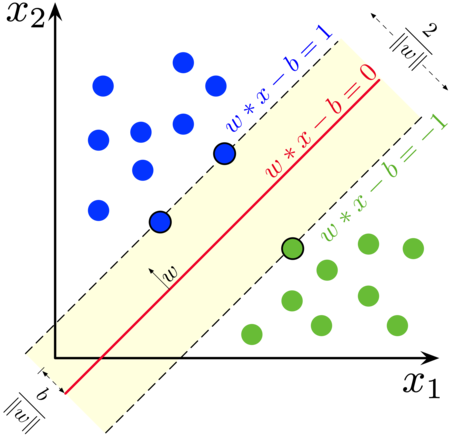
\includegraphics[width=0.3\textwidth]{report-latex/figures/SVM_margin.png}
    \caption{SVM example: Maximum-margin hyperplane and margins for an SVM trained with samples from two classes. Samples on the margin are called the support vectors.}
    \label{fig:SVM_margin}
\end{figure}

Radial basis function kernel (RBF kernel) is a popular kernel function used in various kernelized learning algorithms, which is commonly used in support vector machine classification.

\begin{equation}
    K(x,x') = \exp(-\frac{\norm{x-x'}^2}{2\sigma^2})
\end{equation}

${\norm{x-x'}^2}$ may be recognized as the squared Euclidean distance between the two feature vectors.
$\sigma$ is a free parameter\cite{web:Radial_basis_function_kernel}. 


\subsection{Multinomial Naive Bayes}
The second model we presented here is multinomial naive bayes. Naive bayes is also a supervised learning algorithm. It is a model that commonly used in text classification tasks. Hereby we introduce the principle behinds the algorithm. In multinomial naive bayes\cite{web:Multinomial_Naive_Bayes}, the likelihood of observing a histogram x is given by

\begin{equation}
    p(x|C_k) = \frac{(\Sigma_i x_i)^!}{{\Pi_i x_i}^!} \Pi_i {p_k_i}^{x_i}
\end{equation}

The multinomial naïve bayes classifier becomes a linear classifier when expressed in log-space.

\begin{equation}
\begin{split}
    \log{p(C_k|x)} \propto \log{p(C_k) \Pi^n_{i=1} {p_{ki}}^{x_i}} \\
    &= \log{p(C_k)} + \Sigma^n_{i=1}x_i*log{p_{ki}} \\
    &= b + w^Tx
\end{split}
\end{equation}
where {b=\log p(C_{k})} and {w_{ki}=\log p_{{ki}}}.




\subsection{XGBoost}
The last model we want to introduce here is XGBoost. XGBoost is a widely-used supervised learning algorithm as well. It is a decision-tree-based ensemble algorithm with a gradient boosting framework. Gradient boosting is an approach where new models are created that predict the residuals or errors of prior models and then added together to make the final prediction\cite{web:XGBoost}. When adding the new models, it will minimize the loss by using gradient descent algorithm. Based on this, XGBoost has a regularized objective for better generalization, and additive solution for generic objective function.

For XGBoost\cite{web:XGBoost_LAmeetup}, the object function is
\begin{equation}
    Obj = -\frac{1}{2}\Sigma^{T}_{j=1}\frac{G^2_j}{H_j+\lambda}+\gamma T
\end{equation}

This object function include the training loss and the complexity of trees. The optimal leaf weight is 
\begin{equation}
    w^*_j=\frac{G_j}{H_j+\lambda}
\end{equation}


%-------------------------------------------------
\section{Experiments}
%-------------------------------------------------
In this section, we will show you how we did analysis on our raw data set and how we did data processing to make them more effective when applying our machine learning methods.

\subsection{Dataset}
The data set we use is from Kaggle \cite{web:kaggle}. Twitter Users were evenly selected from Republicans and Democrats. About 200 tweets were collected from each user. Overall, our dataset contains 84,502 tweets with party labels and the labels are roughly balanced.

\begin{table}[h]
\begin{center}
\begin{tabular}{|l|c|c|}
\hline
Party & Handle & Tweet \\
\hline\hline
Republican & 222 & 42434\\
Democrat & 211 & 42068 \\
\hline
Total & 433 & 84502 \\
\hline
\end{tabular}
\end{center}
\caption{This shows the raw data structure.}
\label{tab:raw-data-table}
\end{table}

Table \ref{tab:raw-data-table} shows the raw data structure.

\subsection{Prepossessing Steps}

\subsubsection*{Step 1. Remove Unrelated Characters}

There are some characters that have nothing to do with our classification, such as the twitter handles, punctuation and digits. Figure \ref{fig:raw_example} illustrates the parts we removed in step 1.
\begin{figure}[h]
    \centering
    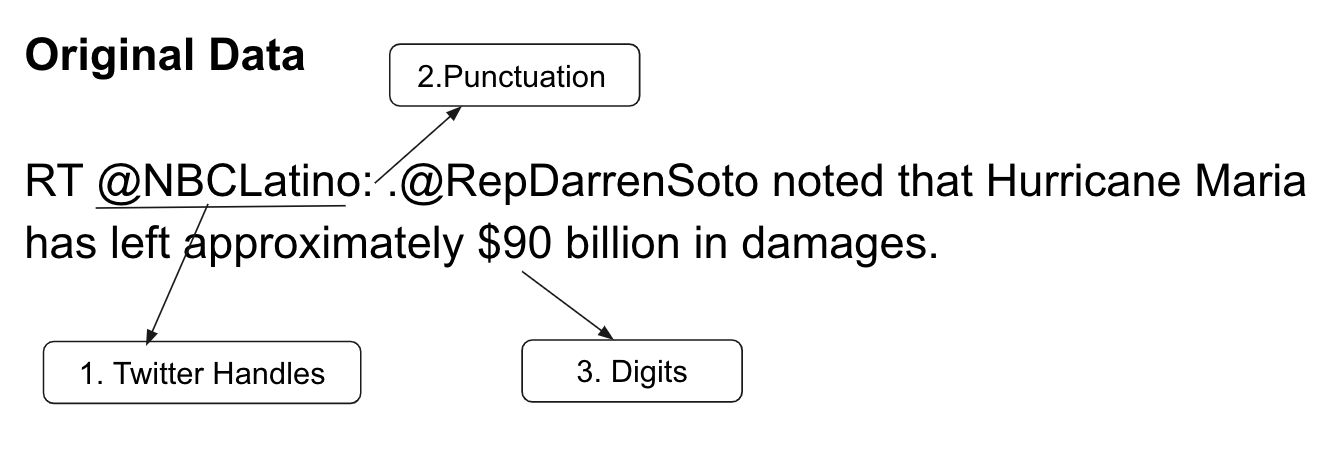
\includegraphics[width=0.5\textwidth]{report-latex/figures/raw_example.png}
    \caption{One example tweet from our data set.}
    \label{fig:raw_example}
\end{figure}

\subsubsection*{Step 2. Tokenization Process and Remove Stop Words}

In this step, we first tokenized strings into separate words. Then, by analyzing the frequency of each words, we found that the words with highest frequencies do not have any meaning and appear very often in both party's tweets. 

\begin{table}[h]
\begin{center}
\begin{tabular}{|c|c|}
\hline
\textbf{word} & \textbf{frequency}\\
\hline\hline
the & 37324\\
to & 28725\\
of &	15877\\
and &	15340\\
in &	13931\\
a &	12087\\
for &	11741\\
rt &	9986\\
on &	9093\\
is &	7476\\
\hline
\multicolumn{2}{| c |}{Republican's Tweets}\\
\hline
\end{tabular}
&
\begin{tabular}{|c|c|}
\hline
\textbf{word} & \textbf{frequency}\\
\hline\hline
the	& 33980\\
to	&	28825\\
of	&	15483\\
and	&	14704\\
a	&	13076\\
in	&	12074\\
for	&	11382\\
rt	&	9068\\
is	&	7651\\
on	&	7642\\
\hline
\multicolumn{2}{| c |}{Democrat's Tweets}\\
\hline
\end{tabular}
\end{center}
\caption{These two tables show the 10 words with highest frequencies in republican's and democrat's tweets respectively.}
\label{tab:raw-data-compare-table}
\end{table}

Table \ref{tab:raw-data-compare-table} compares the 10 words with highest frequencies in republican's and democrat's tweets. We can observe that top 10 words for both party's tweets are the same with slightly difference in the order. All of those high frequency words are just stop words with no meanings. 

\begin{figure}[h]
    \centering
    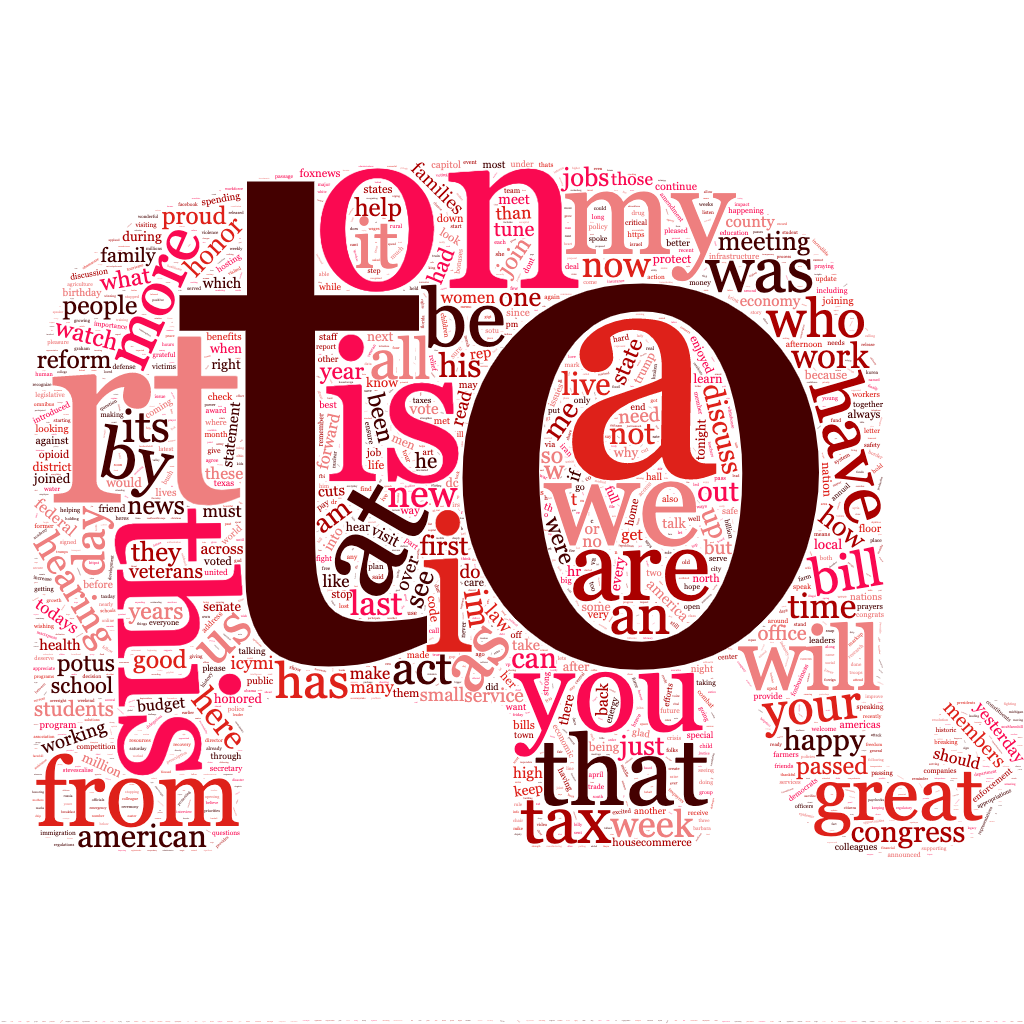
\includegraphics[width=0.5\textwidth]{report-latex/figures/rep_raw.png}
    \caption{A word cloud based on random sampled word frequency of republican party's tweets}
    \label{fig:rep_raw}
\end{figure}

\begin{figure}[h]
    \centering
    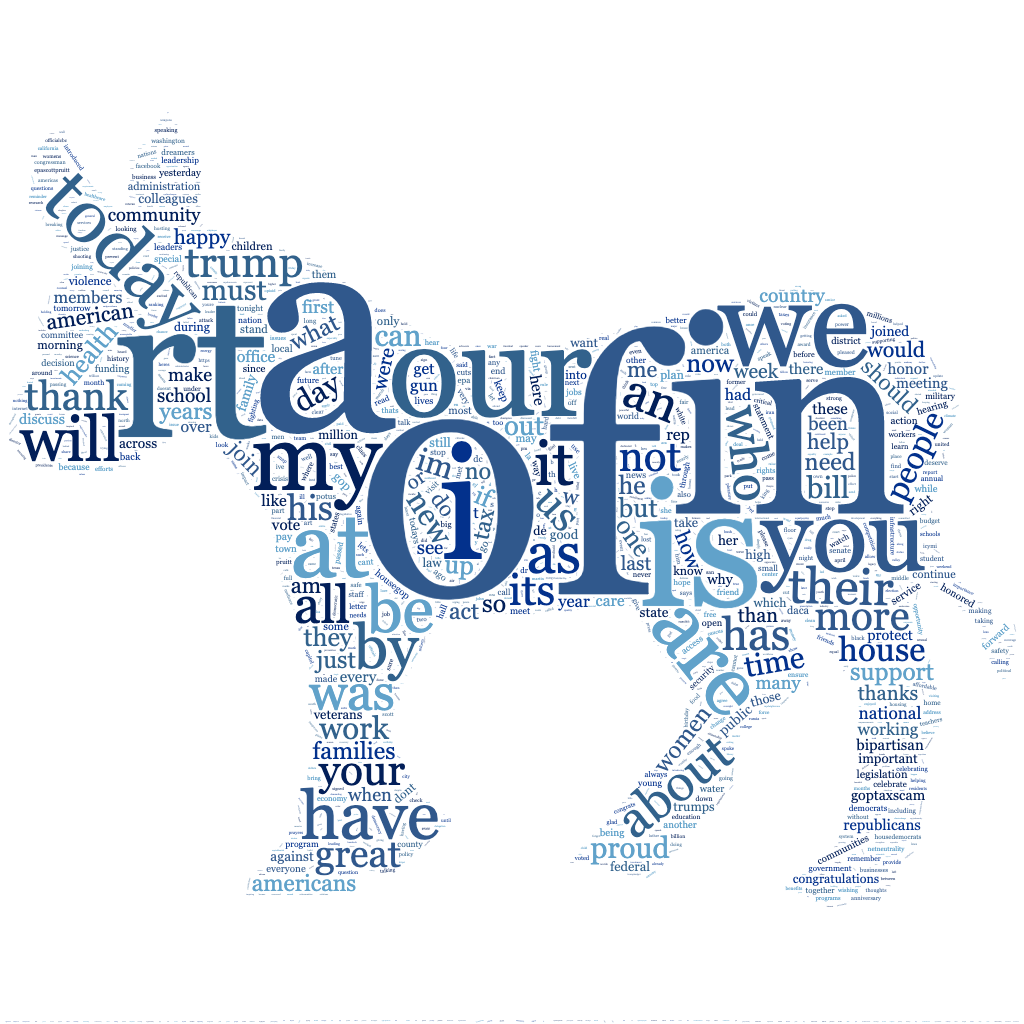
\includegraphics[width=0.5\textwidth]{report-latex/figures/dem_raw.png}
    \caption{A word cloud based on random sampled word frequency of democrat party's tweets}
    \label{fig:dem_raw}
\end{figure}

In Figure \ref{fig:rep_raw} and Figure \ref{fig:dem_raw}, we made random sample over the party's data respectively. This time we can observe some high frequency words with meanings such as "great" and "today". However, it is clear to see that the words with highest frequencies are still those uninformative stop words, such as "to" or "of". We removed those stop words using the stop word library.

One thing to notice, there is another stop word that is not in our usual stop words library here, which is "RT". It appears very often as the beginning string of our collected tweets (in the left side of both Figure \ref{fig:rep_raw} and Figure \ref{fig:dem_raw}). Thus, we removed "RT" as the last part of step 2.

\subsubsection*{Step 3. Stemming Process}

By stemming the tokenized words, we made our data more dense and reduce the dimension.

Here, Table \ref{tab:stemmed-table} displays the output based on the previous steps. The data output of this step are considered clean.

\begin{table}[H]
\begin{center}
\begin{tabular}{|p{0.1\textwidth}|p{0.3\textwidth}|}
\hline
\textbf{Steps} & \textbf{Output} \\
\hline\hline
Raw data & {Today, Senate Dems vote to \#SaveTheInternet.}\\
\hline
Remove unrelated characters & {Today Senate Dems vote to SaveTheInternet}\\
\hline
Tokenization & {[Today, Senate, Dems, vote, to, SaveTheInternet]}\\
\hline
Remove stop words & {[Today, Senate, Dems, vote, SaveTheInternet]}\\
\hline
Stemming & {[today, senate, dem, vote, savetheinternet]}\\
\hline
\end{tabular}
\end{center}
\caption{This shows the output of each steps.}
\label{tab:stemmed-table}
\end{table}

\subsubsection*{Step 4. Join back the Tokenized Words}

In order to treat every word as a feature, we want to vectorize them. However, the vectorization function TfidVectorizer we want to use requires corpus as input. Thus, in this step, we join back our tokenized words.

Here is an example. Suppose we have only limited word space ([today, tax, student, senate, trump, dem, vote, biden, savetheinternet]), and we use the previous cleaned tweet in table  \ref{tab:stemmed-table} as corpus: "today senate dem vote savetheinternet".

The following table \ref{tab:tf-idf-table} illustrate how words are processed into features:

\begin{table}[H]
\begin{center}
\begin{tabular}{||c|c||}
\hline
word space/features & value\\
\hline\hline
today & 1 \\
\hline
tax & 0 \\
\hline
student & 0\\ 
\hline
senate & 1 \\
\hline
trump & 0\\
\hline
dem & 1\\
\hline
vote & 1\\
\hline
biden & 0\\
\hline
savetheinternet & 1\\
\hline
\end{tabular}
\end{center}
\caption{This shows the value of one tweet entry toward the whole word space.}
\label{tab:tf-idf-table}
\end{table}

\subsection{Software, Tools and Resources}

\subsubsection*{Data Source}
\begin{itemize}
  \item Our data set Democrat Vs Republican Tweets was retrieved from Kaggle\cite{web:kaggle}
\end{itemize}

\subsubsection*{Data Preparation}
\begin{itemize}
  \item The basic software we used for preliminary data analysis is R Studio.
  \item The word clouds were generated on \url{https://www.wordclouds.com} with the customized word frequency lists. 
\end{itemize}

\subsubsection*{Machine Learning}
\begin{itemize}
  \item Jupyter Notebook
\end{itemize}

\subsubsection*{Version Control}
\begin{itemize}
  \item Github was used for version control of the code.
  \item Overleaf and Google Doc were used for documentation purpose. 
\end{itemize}


\subsection{Hardware}
Some machine learning methods we used took a very long time to run. In this case, some of the procedures were done separately on laptops that have the higher performance.

Machine models:
\begin{itemize}
  \item Macbook Pro 15” 2018
  \item Dell XPS13 
\end{itemize}

%-------------------------------------------------
\section{Results and Discussion}
%-------------------------------------------------

\subsection{Model Training and Hyper-parameter Tuning}
\subsubsection{Multinomial Naive Bayes}
For the multinomial Naive Bayes model.We ran a grid search on the parameter alpha. The result is showing in the following graph.

\begin{figure}[h]
    \centering
    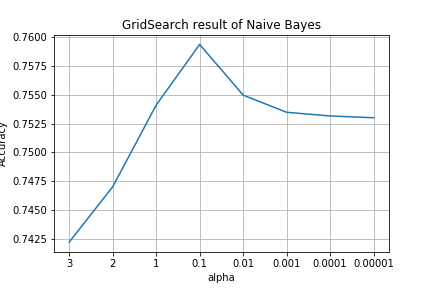
\includegraphics[width=0.5\textwidth]{report-latex/figures/NB_gs.png}
    \caption{The Grid Search Result for Naive Bayes}
    \label{fig:NB_gs}
\end{figure}

The grid search result shows that when $alpha = 0.1$, our model performs the best. Therefore, we choose the model with $alpha = 0.1$ The accuracy of 4-fold cross validation is 75.94\% eventually.

\subsubsection{Support Vector Machine}
According to this post (KOWALCZYK et al., 2020) \cite{kowalczyk_alexandre}, linear kernel support vector machine works the best for text classification tasks. Therefore, we chose linear kernel for our tasks. If linear kernel was chosen, then the only hyper-parameter that has significant impact to our model is C.
To find the best hyper-parameters for our model, we ran a grid search on the parameter C. The result is showing in the following graph.
\begin{figure}[h]
    \centering
    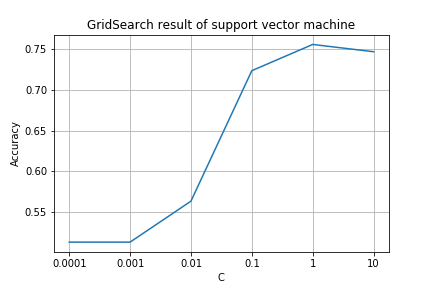
\includegraphics[width=0.5\textwidth]{report-latex/figures/SVM_gs.png}
    \caption{The Grid Search Result for Support Vector Machine}
    \label{fig:SVM_gs}
\end{figure}

The grid search result on C shows that when $C = 1$ our model performs the best, therefore, we choose $C = 1$ for our final model for support vector machine. The accuracy of 4-fold cross validation is 75.94\% eventually.

\subsubsection{XGBoost}
For XGBoost, we have more hyper-parameters to test than the previous two models. Consider that the training time cost is expensive, we decided to ran a random search on the hyper-parameters follows the set up as below.

\begin{center}
 \begin{tabular}{||c c||} 
 \hline
 Hyper-Parameters & Value Range  \\ [0.5ex] 
 \hline\hline
 max-depth & [5,6,7,8,9,10] \\ 
 \hline
 min-child-weight & [0-10]\\
 \hline
 eta & [0-2] \\
 \hline
\end{tabular}
\end{center}

The result of the random search shows as below:

\begin{center}
 \begin{tabular}{||c c c c||} 
 \hline
 max_depth & min-child-weight & eta & accuracy  \\ [0.5ex] 
 \hline\hline
 7 & 2.27 & 1.39 &0.7035  \\ 
 \hline
 8 & 4.91 & 1.1 & 0.707 \\ 
 \hline
 6 & 6.8 & 1.5 & 0.695 \\
 \hline
 6 & 1.2 & 4.0 &  0.698\\
 \hline
 6 & 4.3 & 1.06 &  0.698\\
 \hline
 5 & 5.9 & 1.2 &  0.691\\
 \hline
 8 & 1.2 & 1.7 &  0.71\\
 \hline
 9 & 4.2 & 1.03 &  0.694\\
 \hline
 6 & 7.4 & 0.59 &  0.695\\
 \hline
 6 & 6.5 & 0.71 &  0.694\\
 \hline
 
 \hline
\end{tabular}
\end{center} 

In general we can see a pattern a here that higher max depth tends to yield model with high accuracy. Min child weight around 1 tends to improve the model accuracy. Based off our observation, we trained our final with the XGBoost model with the following hyper-parameters.

\begin{center}
 \begin{tabular}{||c c c||} 
 \hline
 Max-Depth & Min-Weight & Eta  \\ [0.5ex] 
 \hline\hline
 10 & 4.27 & 1.06 \\
 \hline
\end{tabular}
\end{center}

\subsection{Model Evaluation and Selection}
After we improved the performance of each model by hyper-parameter tuning, we present the test results for each model with the final selected hyper-parameters. The result shows in the figure below:

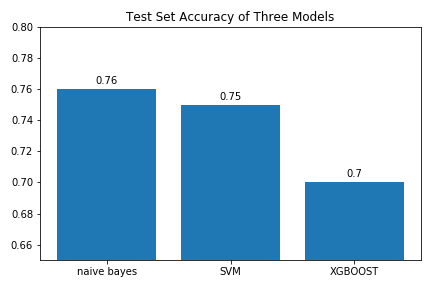
\includegraphics[width=0.5\textwidth]{report-latex/figures/TEST_ALL.png}

The result shows that support vector machine and Naive Bayes perform much better than XGBoost model. However, we don't see a large difference between the performance of Naive Bayes and support vector machine, although Naive Bayes performs slightly better than the Support Vector Machine. We want to further understand which model to choose. 

\subsubsection{McNemar's Test on Naive Bayes and Support Vector Machine}
Due to the similar performance, we want to understand if the Naive Bayes model is the same as the support vector machine model. Then we run a McNemar's test between these two models.
\newline
\newline
The confusion matrix of Naive Bayes model is shown as below:
\newline
\begin{tabular}{l|l|c|c|c}
\multicolumn{2}{c}{}&\multicolumn{2}{c}{Support Vector Machine}&\\
\cline{3-4}
\multicolumn{2}{c|}{}&Positive&Negative&\multicolumn{1}{c}{Total}\\
\cline{2-4}
\multirow{Naive Bayes}& Positive & $6758$ & $1222$ & $7980$\\
\cline{2-4}
& Negative & $1056$ & $8256$ & $9312$\\
\cline{2-4}
\multicolumn{1}{c}{} & \multicolumn{1}{c}{Total} & \multicolumn{1}{c}{$9814$} & \multicolumn{    1}{c}{$9748$} & \multicolumn{1}{c}{$17292$}\\
\end{tabular}

After we ran the McNemar's test over two model's prediction, we have p-value of 0.001. Therefore, we reject the null hypopthesis which states that the two model are the same. We conclude that the two models are fundamentally different. 

\subsubsection{Metrics}
We want to further investigate what are the differences between the two models. We use confusion matrix to learn more about the pattern of the two models. We assume that 'Republican' is labeled as positive, and vice versa.

\begin{figure}[!htb]
\minipage{0.23\textwidth}
  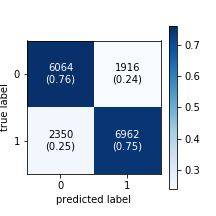
\includegraphics[width=\linewidth]{report-latex/figures/svm_cm.png}
  \caption{Confusion Matrix of svm}\label{fig:svm_cm}
\endminipage\hfill
\minipage{0.23\textwidth}
  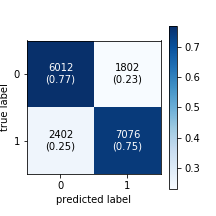
\includegraphics[width=\linewidth]{report-latex/figures/nb_cm.png}
  \caption{Confusion Matrix of Naive Bayes}\label{fig:nb_cm}
\endminipage\hfill
\end{figure}

The confusion matrix didn't reveal us any significant differences on traits among two models. Therefore, we try to use Accuracy, Precision, Recall, F1, and MCC metrics to further investigate the traits of the models.

\begin{center}
 \begin{tabular}{|| l ||c | c ||} 
 \hline
 Metric & Naive Bayes &  SVM\\ [0.5ex] 
 \hline\hline
 Accuracy & 0.757   & 0.753 \\ 
 \hline
 Precision & 0.747 & 0.748 \\
 \hline
 Recall & 0.797 & 0.784 \\
 \hline
 F1 & 0.771 & 0.765 \\
 \hline
 MCC & 0.514 & 0.506 \\ [1ex] 
 \hline
\end{tabular}
\end{center}

From the above table, we can see that Naive Bayes has noticeable higher recall rate, F1 score, and MCC. Since we assigned "Repulican" as our model, higher recall rate and F1-score can be interpreted as Naive Bayes model has better performance when identifying Republican tweets than the Support Vector Machine model. This feature can potentially be useful when performing certain types of task targeting republican tweets.  The higher MCC also indicates that our model has a strong positive correlation to the test set. The above information told us that our model, in general, is better at predicting Republican tweets than Democratic tweets. Between two models, there is no significant difference among their prediction patterns.

Besides, Naive Bayes is way more faster to train than support vector machine when the number of features is huge. 


%-------------------------------------------------
\section{Conclusions}
%-------------------------------------------------

After experimenting three types of models on performing political text classification, we conclude that Naive Bayes will be our final model. Naive Bayes has the highest accuracy of 76\% on our test data set, and the high recall rate of Naive Bayes model allow us to do some potential future works based on such a model. Besides, Naive Bayes model also has lower training and predicting cost, which is potentially useful in industrial applications.  

%-------------------------------------------------
\section{Acknowledgements}
%-------------------------------------------------

Thanks to Kyle Pastor who contributed to the initial data set on Kaggle\cite{web:kaggle}. We also appreciate the discussion posts about that data set, which inspired us a lot. 

%-------------------------------------------------
\section{Contributions}
%-------------------------------------------------
\subsubsection*{Computational Task}
\begin{itemize}
  \item Han is responsible for data prepossessing, researching and implementing a machine learning pipeline
  \item Siyi is responsible for developing and tuning the models
  \item Qiwen is responsible for evaluating the model
\end{itemize}

\subsubsection*{Visualization Task}
\begin{itemize}
  \item Han is responsible for machine learning methods.
  \item Siyi is responsible for data set statistics.
  \item Qiwen is responsible for the rest.
\end{itemize}

\subsubsection*{Documentation Task}
\begin{itemize}
  \item Han is responsible for methods of the model, results and conclusion
  \item Qiwen is responsible for the introduction and related work
  \item Siyi is responsible for the experiment and the rest
\end{itemize}


{\small
\bibliographystyle{ieee}
\bibliography{bibliography.bib}
}

\end{document}
